\subsection{Moto Circolare}

\subsubsection{Formule}

\setcounter{equation}{0}

La "\textit{Legge oraria}":

\begin{equation}
\theta=\theta_0+\omega\cdot t
\end{equation}

Frequenza e periodo:

\begin{equation}
\begin{array}{ll}
\textrm{Frequenza }f=\frac{1}{T} \\
\\
\textrm{Periodo }T=\frac{1}{f}
\end{array}
\end{equation}

Velocità angolare:

\begin{equation}
\omega=\frac{2\pi}{T} = 2\pi f
\end{equation}

Velocità tangenziale:

\begin{equation}
v=\frac{
2\pi r
}{
T
}
\end{equation}

Accelerazione centripeta:


\begin{equation}
a_c=\frac{v^2}{r}=\omega^2 r
\end{equation}




\subsubsection{Esercizi}

\begin{enumerate}

\item{Due pesi con attrito} \label{ex_2pca}


\begin{figure}[h]
\centering
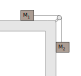
\includegraphics[width=0.6\textwidth]{carrucole.4.pdf}
\end{figure}

In the system shown above, the block of mass $M_1$, is on a rough horizontal table.

The string that attaches it to the block of mass $M_2$ passes over a frictionless pulley of negligible mass.

The coefficient of kinetic friction $\mu_k$ between $M_1$ and the table is less than the coefficient of static friction $\mu_s$.

\begin{enumerate}
\item On the diagram below, draw and identify all the forces acting on the block of mass $M_1$
\begin{figure}[h]
\centering
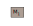
\includegraphics[width=0.4\textwidth]{carrucole.5.pdf}
\end{figure}
\item In terms of $M_1$ and $M_2$ determine the minimum value of $\mu_s$ that will prevent the blocks from moving

\vspace{1cm}
The blocks are set in motion by giving $M_2$ a momentary downward push.  In terms of $M_1$, $M_2$, $\mu_k$ and $g$, determine each of the following:

\item The magnitude of the acceleration of $M_1$
\item The tension of the string
\end{enumerate}

Soluzione a pagina \pageref{s_2pca}

\end{enumerate}

\subsubsection{Multiple choice} \label{q_mcmc}

Soluzioni a pagina \pageref{s_mcmc}

\begin{enumerate}


\item 

A ball is fastened to a string and is swung in a vertical circle. When the ball is at the
highest point of the circle its velocity and acceleration directions are:

\begin{figure}[H]
\centering
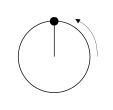
\includegraphics[width=0.4\textwidth]{rot-ex-1.pdf}
\end{figure}

\begin{figure}[h]

\centering

\begin{minipage}{.1\textwidth}
  \centering
  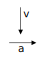
\includegraphics[width=\linewidth]{rot-ex-1a.pdf}
  A
\end{minipage}
\hspace{1cm}
\begin{minipage}{.1\textwidth}
  \centering
  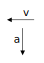
\includegraphics[width=\linewidth]{rot-ex-1b.pdf}
  B
\end{minipage}
\hspace{1cm}
\begin{minipage}{.1\textwidth}
  \centering
  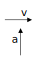
\includegraphics[width=\linewidth]{rot-ex-1c.pdf}
  C
\end{minipage}
\hspace{1cm}
\begin{minipage}{.1\textwidth}
  \centering
  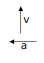
\includegraphics[width=\linewidth]{rot-ex-1d.pdf}
  D
\end{minipage}
\end{figure}

\item A ball with a mass m is fastened to a string and is swung in a vertical circle. 

(see previous picture for setup)

When the ball is at the highest point of the circle the tension in the string is:

\begin{itemize}
\item[A] $mg$
\item[B] $mg + ma$
\item[C] $ma ‐mg$ 
\item[D] $mg/ma$
\end{itemize}

\item An object, shown in the accompanying figure, moves in uniform circular motion.

Which arrow best depicts the net force acting on the object at the instant shown?

\begin{figure}[H]
\centering
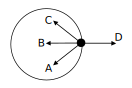
\includegraphics[width=0.4\textwidth]{rot-ex-3.pdf}
\end{figure}


\item A motorcyclist moves at a constant speed down one hill and up another hill along the smooth curved surface. 

\begin{figure}[H]
\centering
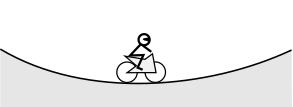
\includegraphics[width=0.6\textwidth]{mot-ex-4.pdf}
\end{figure}

When the motorcyclist reaches the lowest point of the curve its velocity and acceleration directions are:



\begin{figure}[H]

\centering

\begin{minipage}{.1\textwidth}
  \centering
  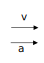
\includegraphics[width=\linewidth]{mot-ex-4a.pdf}
  A
\end{minipage}
\hspace{1cm}
\begin{minipage}{.1\textwidth}
  \centering
  \includegraphics[width=\linewidth]{mot-ex-4b.pdf}
  B
\end{minipage}
\hspace{1cm}
\begin{minipage}{.1\textwidth}
  \centering
  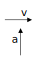
\includegraphics[width=\linewidth]{mot-ex-4c.pdf}
  C
\end{minipage}
\hspace{1cm}
\begin{minipage}{.1\textwidth}
  \centering
  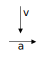
\includegraphics[width=\linewidth]{mot-ex-4d.pdf}
  D
\end{minipage}
\end{figure}

\item A car moves along the curved track. 

\begin{figure}[H]
\centering
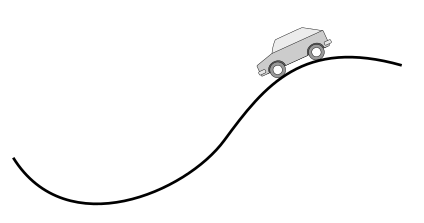
\includegraphics[width=0.6\textwidth]{rot-ex-4.pdf}
\end{figure}

What is the apparent weight of the driver when the car reaches the lowest point of the curve?

\begin{itemize}
\item[A] $mg$
\item[B] $mg+ma$
\item[C] $ma-mg$ 
\item[D] $mg/ma$
\end{itemize}

\item Acar moves along the curved track (same situation as the previous question).

What is the direction of $F_N$ of the driver when the car reaches the lowest point of the curve?

\begin{itemize}
\item[A] Upward
\item[B] Downward
\item[C] Forward
\item[D] Backward
\end{itemize}


\item A car is traveling on a road in hilly terrain, see figure above.
Assume the car has speed $v$ and the tops and bottoms of the hills have radius of curvature $R$.
The driver of the car is most likely to feel weightless:

\begin{itemize}
\item[A] at the top of a hill when $v = \sqrt{gR}$
\item[B] at the bottom of a hill when $v > \sqrt{gR}$
\item[C] going down a hill when $v = \sqrt{gR}$
\item[D] at the top of a hill when $v < \sqrt{gR}$
\end{itemize}

\vspace{1cm}

A 0.2 kg ball rotates at a constant speed of 3 $\frac{m}{s}$ on the end of 1.2 m long string.

The string describes a horizontal circle.

\begin{figure}[H]
\centering
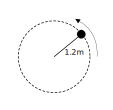
\includegraphics[width=0.3\textwidth]{rot-ex-5.pdf}
\end{figure}

\item What is the centripetal acceleration of the object?

\begin{itemize}
\item[A] $1.2 \frac{m}{s^2}$
\item[B] $3.0 \frac{m}{s^2}$
\item[C] $7.5 \frac{m}{s^2}$
\item[D] $3.2 \frac{m}{s^2}$
\end{itemize}


\item What is the centripetal force exerted on the object?

\begin{itemize}
\item[A] $1.0 N$
\item[B] $1.2 N$
\item[C] $0.2 N$
\item[D] $1.5 N$
\end{itemize}


\item When a student stands on a rotating table, the frictional force exerted on the student by the table is

\begin{itemize}
\item[A] greater in magnitude than the frictional force exerted on the table by the student
\item[B] less in magnitude than the frictional force exerted on the table by the student
\item[C] equal in magnitude than the frictional force exerted on the table by the student
\item[D] directed away from the center of the table
\end{itemize}


\item A child whirls a ball at the end of a rope, in a uniform circular motion. 

Which of the following statements is NOT true?

\begin{itemize}
\item[A] The speed of the ball is constant.
\item[B] The velocity of the ball is constant.
\item[C] The radius is constant
\item[D] The magnitude of the ball’s acceleration is constant.
\end{itemize}



\item The horizontal table rotates at a constant speed. 

As viewed from above, a coin on the table moves counterclockwise in a circle.



\begin{figure}[H]
\centering
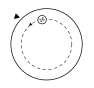
\includegraphics[width=0.4\textwidth]{rot-ex-12.pdf}
\end{figure}

Which of the following vectors best represents the direction of the frictional force 
exerted on the coin by the table when the coin is in the position shown?

\begin{figure}[H]

\centering

\begin{minipage}{.1\textwidth}
  \centering
  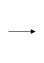
\includegraphics[width=\linewidth]{rot-ex-12a.pdf}
  A
\end{minipage}
\hspace{1cm}
\begin{minipage}{.1\textwidth}
  \centering
  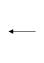
\includegraphics[width=\linewidth]{rot-ex-12b.pdf}
  B
\end{minipage}
\hspace{1cm}
\begin{minipage}{.1\textwidth}
  \centering
  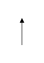
\includegraphics[width=\linewidth]{rot-ex-12c.pdf}
  C
\end{minipage}
\hspace{1cm}
\begin{minipage}{.1\textwidth}
  \centering
  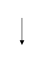
\includegraphics[width=\linewidth]{rot-ex-12d.pdf}
  D
\end{minipage}
\end{figure}

\item A centripetal force $F$ is applied to an eraser moving at a constant speed $v$ in a horizontal circle of radius $r$.

If the same force is applied, but the radius is halved, what happens to the speed of the eraser?

\begin{itemize}
\item[A] Increased by a factor of $2$
\item[B] decreased by a factor of $2$  
\item[C] increased by a factor of $\sqrt{2}$  
\item[D] decreased by a factor of $\sqrt{2}$
\end{itemize}

\item A centripetal force $F$ is applied to an object moving at a constant speed $v$
in a horizontal circle of radius $r$.

If the radius is quadrupled and the speed is doubled, what happens to the centripetal force?

\begin{itemize}
\item[A] Increased by a factor of $2$
\item[B] decreased by a factor of $2$
\item[C] doesn’t change
\item[D] increased by a factor of $\sqrt{2}$
\end{itemize}


The diagram below is a snapshot of three cars all moving counterclockwise during a 
one lap race on an elliptical track.  


\begin{figure}[H]
\centering
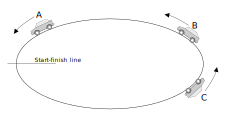
\includegraphics[width=0.6\textwidth]{rot-ex-15.pdf}
\end{figure}


\item Which car the moment of the snapshot has the smallest displacement?

\begin{itemize}
\item[A] car A
\item[B] car B
\item[C] car C
\item[D] all three cars have the same displacement 
\end{itemize}

\item Which car at the moment of the snapshot must have none zero acceleration?

\begin{itemize}
\item[A] car A
\item[B] car B
\item[C] car C
\item[D] all three cars have none zero acceleration
\end{itemize}


\item Which car can at the moment of the snapshot must have a centripetal force directed to the center of the center of the curvature?

\begin{itemize}
\item[A] car A
\item[B] car B
\item[C] car C
\item[D] all three cars must have the centripetal force directed to the center of the curvature
\end{itemize}


\item A roller coaster car is on a track that forms a circular loop of radius $R$ in the vertical plane.
If the car is to just maintain contact with track at the top of the loop, 
what is the minimum value for its velocity at this point? 

\begin{itemize}
\item[A] $gR$
\item[B] $0.5gR$
\item[C] $2gR$
\item[D] $(gR)^{\frac{1}{2}}$
\end{itemize}

\item A coin rests on a turntable a distance $r$ from the axis of rotation.
The turntable rotates with a constant speed of $v$.
What is the minimum coefficient of static friction between the turntable and the coin?

\begin{itemize}
\item[A] $v^2rg$
\item[B] $\frac{v^2}{rg}$
\item[C] $\frac{rg}{v^2}$
\item[D] $\frac{v^2}{r}$
\end{itemize}


\item A car goes around a curve of radius $r$ at a constant speed $v$.
The coefficient of static friction between the tires and the surface is $\mu$.
What is the maximum value of the car’s velocity in order to prevent car from skidding of the road? 
 
\begin{itemize}
\item[A] $\mu rg$
\item[B] $\frac{\mu r}{g}$
\item[C] ${\mu µrg}^2$
\item[D] $\frac{g}{\mu r}$
\end{itemize}



\end{enumerate}

